% === B02 - SIMD Conversiones Shuffle Blend ===
% David Alejandro Gonzalez Marquez
% dmarquez@dc.uba.ar / fokerman@gmail.com
% https://github.com/fokerman/Orga2Course

\documentclass[aspectratio=169]{beamer}
% \documentclass[handout]{beamer}

% % % Packages
\usepackage[sfdefault]{AlegreyaSans}
\usepackage{inconsolata}
\usepackage{multicol}
\usepackage{multirow}
\usepackage[spanish]{babel}
\usepackage[utf8]{inputenc}
\usepackage{enumerate}
\usepackage{color}
\usepackage{xcolor}
\usepackage[absolute,overlay]{textpos}
  \setlength{\TPHorizModule}{1mm}
  \setlength{\TPVertModule}{1mm}
\usepackage{framed}
\usepackage{mfirstuc} % para poner en mayusculas la primer letra
\usepackage{xspace} % para crear espacios en comandos 
\usepackage{pbox}
\usepackage{tikz}
\usepackage{mathabx}

% % % Beamer config
\usetheme{Pittsburgh}
\usecolortheme[rgb={1,0.48,0.0}]{structure}
\setbeamercolor{block title}{fg=white,bg=verdeuca}
\xdefinecolor{verdeuca}{rgb}{0.0,0.48,0.54}
\xdefinecolor{naranjauca}{rgb}{1,0.48,0.0}
\setbeamercolor{palette quaternary}{fg=white,bg=verdeuca}
\setbeamertemplate{title page}[default][colsep=-4bp, rounded=true] % remove title shadow
\setbeamertemplate{frametitle}[default][colsep=-2bp, shadow=false] % remove frame title shadow
\setbeamertemplate{navigation symbols}{} % remove navigation symbols
\beamertemplatenavigationsymbolsempty

% % % Colors
\definecolor{AzulClaro}{rgb}{.31,.506,.741}
\definecolor{Gris}{gray}{0.8}
\definecolor{Celeste}{rgb}{.255,.41,.884}
\definecolor{Rojo}{rgb}{1, 0, 0}
\definecolor{a}{rgb}{0.0, 0.53, 0.74}
\definecolor{r}{rgb}{0.89, 0.0, 0.13}
\definecolor{v}{rgb}{0.0, 0.5, 0.0}
\definecolor{y}{rgb}{0.0, 0.5, 0.5}

% % % Rename
\newcommand{\tab}[0]{\hspace{15pt}}

% % % Blocks
\setbeamercolor{block body}{fg=black, bg=black!10}
\setbeamercolor{block title}{fg=black, bg=black!20}
\setbeamercolor{coloredboxstuffNaranja}{fg=naranjauca,bg=black!10} %% PARA LOS BOX
\setbeamercolor{coloredboxstuffVerde}{fg=verdeuca,bg=black!10} %% PARA LOS BOX

% % % Start

\title{\Huge SIMD Parte 2}
\subtitle{Conversiones, Shuffles y Blends}
      
\author{David Alejandro González Márquez}
\institute{Departamento de Computación\\
Facultad de Ciencias Exactas y Naturales\\
Universidad de Buenos Aires}
\date{}

\begin{document}

\begin{frame}[plain]
  \titlepage
\end{frame}

\begin{frame}
	\frametitle{Agenda}
	\Large
	\begin{itemize}
	\item[-] Problemas de Precisión
	\vskip 10pt
	\item[-] Instrucciones de Shuffle
	\vskip 10pt
	\item[-] Instrucciones de Blend
	\vskip 10pt
	\item[-] Instrucciones de Conversión
	\end{itemize}
\end{frame}

\begin{frame}[fragile]
	\frametitle{Problemas de Precisión}
	\begin{itemize}
	\item[-] No todos los números pueden ser representados de \textbf{forma exacta} en punto flotante\\
	\vspace{0.3cm}
	\pause
	\colorbox{verdeuca}{ \begin{minipage}{12cm} \small \textcolor{white}{
	\footnotesize \textbf{Por ejemplo}: El número $1.1$ no puede ser representado en Float de forma exacta,\\  siendo el más aproximado: $1.100000023841858$}
	\normalsize \end{minipage}}
	\pause
	\vspace{0.3cm}
	\item[-] Las operaciones en enteros no necesariamente generan resultados que caben en un entero del mismo tamaño\\
	\vspace{0.3cm}
	\pause
	\colorbox{verdeuca}{ \begin{minipage}{12cm} \small \textcolor{white}{
	\footnotesize \textbf{Por ejemplo}: La operación en bytes $0xFE \cdot 0x10$ da como resultado $0x0FE0$, no entra en un byte}
	\normalsize \end{minipage}}
	\pause
	\vspace{0.3cm}
	\item[-] Incluso es muy simple perder precisión si nuestros datos temporales son enteros\\
	\vspace{0.3cm}
	\pause
	\colorbox{verdeuca}{ \begin{minipage}{12cm} \small \textcolor{white}{
	\footnotesize \textbf{Por ejemplo}: Si hacemos la operación $(0xFE + 0x11) / 0x02$ en enteros, el resultado es $0x87$,\\ siendo el correcto $0x87,8$ }
	\normalsize \end{minipage}}
	\end{itemize}
\end{frame}

\begin{frame}[fragile]
	\frametitle{Problemas de Precisión}
	\textbf{Moraleja},\\
	\begin{itemize}
	 \vskip 7pt \item[-] Antes de hacer cualquier cálculo, \textbf{analizar} detalladamente los pasos a realizar
	 \pause
	 \vskip 7pt \item[-] Entender cuándo se \textbf{pierde precisión} y decidir qué hacer al respecto
	 \pause
	 \vskip 7pt \item[-] Las operaciones en enteros son \textbf{exactas} en enteros
	 \pause
	 \vskip 7pt \item[-] Las operaciones en punto flotante son siempre \textbf{aproximadas}
	 \pause
	 \vskip 7pt \item[-] Las operaciones de conversión son \textbf{muy costosas}
	 \pause
	 \vskip 7pt \item[-] Los registros tienen un tipo de datos oculto al programador, usar instrucciones en enteros en punto flotante o a la inversa, implica una \textbf{penalidad}
	 \pause
	 \vskip 7pt \item[-] El \textbf{costo} de las operaciones depende de cada una, ya sea en punto flotante o enteros
	\end{itemize}
\end{frame}

\begin{frame}[fragile,t]
	\frametitle{Shuffles}
	Las instrucciones de \emph{Shuffle} permiten \textbf{reordenar} datos en registros.\\
	Sus parámetros serán el \textbf{registro a reordenar} y una \textbf{máscara} que indicará cómo hacerlo.
	\vskip 10pt
	\pause
	\begin{itemize}
	 \item[-] P{\color{a}{SHUF}}{\color{v}{B}} - {\color{a}{Shuf}}fle Packed {\color{v}{B}}ytes
	 \item[-] P{\color{a}{SHUF}}{\color{orange}{H}}{\color{v}{W}} - {\color{a}{Shuf}}fles {\color{orange}{high}} {\color{v}{16bit}} values
	 \item[-] P{\color{a}{SHUF}}{\color{orange}{L}}{\color{v}{W}} - {\color{a}{Shuf}}fles {\color{orange}{low}} {\color{v}{16bit}} values
	 \item[-] P{\color{a}{SHUF}}{\color{v}{D}} - {\color{a}{Shuf}}fle Packed {\color{v}{D}}oublewords
	\end{itemize}
	\begin{itemize}
	 \item[-] {\color{a}{SHUF}}{\color{r}{P}}{\color{v}{S}} - {\color{a}{Shuf}}fle {\color{r}{P}}acked {\color{v}{S}}ingle FP Values
	 \item[-] {\color{a}{SHUF}}{\color{r}{P}}{\color{v}{D}} - {\color{a}{Shuf}}fle {\color{r}{P}}acked {\color{v}{D}}ouble FP Values
	\end{itemize}
\end{frame}

\begin{frame}[fragile,t]
	\frametitle{Shuffles}
	\begin{textblock}{500}(25,5)
	\only<1->{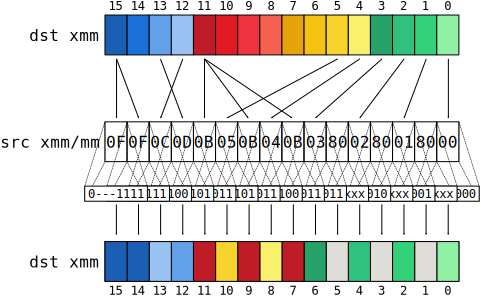
\includegraphics[width=13cm]{img/PSHUFB.png}}
	\end{textblock}
	\begin{textblock}{500}(25,50)
	\only<2->{\includegraphics[scale=0.35]{img/PSHUFB_code.png}}
	\end{textblock}
\end{frame}

\begin{frame}[fragile,t]
	\frametitle{Ejemplo - \texttt{PSHUFB dst, src}}
	\begin{textblock}{500}(30,20) \only<1-18>{\includegraphics[scale=0.7]{img/PSHUFB-layer1.pdf}} \end{textblock}  % fondo
	\begin{textblock}{500}(30,20) \only<2>{\includegraphics[scale=0.7]{img/PSHUFB-layer2.pdf}} \end{textblock}  % 0
	\begin{textblock}{500}(30,20) \only<3>{\includegraphics[scale=0.7]{img/PSHUFB-layer3.pdf}} \end{textblock}  % 1
	\begin{textblock}{500}(30,20) \only<4>{\includegraphics[scale=0.7]{img/PSHUFB-layer4.pdf}} \end{textblock}  % 2
	\begin{textblock}{500}(30,20) \only<5>{\includegraphics[scale=0.7]{img/PSHUFB-layer5.pdf}} \end{textblock}  % 3
	\begin{textblock}{500}(30,20) \only<6>{\includegraphics[scale=0.7]{img/PSHUFB-layer6.pdf}} \end{textblock}  % 4
	\begin{textblock}{500}(30,20) \only<7>{\includegraphics[scale=0.7]{img/PSHUFB-layer7.pdf}} \end{textblock}  % 5
	\begin{textblock}{500}(30,20) \only<8>{\includegraphics[scale=0.7]{img/PSHUFB-layer8.pdf}} \end{textblock}  % 6
	\begin{textblock}{500}(30,20) \only<9>{\includegraphics[scale=0.7]{img/PSHUFB-layer9.pdf}} \end{textblock}  % 7
	\begin{textblock}{500}(30,20) \only<10>{\includegraphics[scale=0.7]{img/PSHUFB-layer10.pdf}} \end{textblock} % 8
	\begin{textblock}{500}(30,20) \only<11>{\includegraphics[scale=0.7]{img/PSHUFB-layer11.pdf}} \end{textblock} % 9
	\begin{textblock}{500}(30,20) \only<12>{\includegraphics[scale=0.7]{img/PSHUFB-layer12.pdf}} \end{textblock} % A
	\begin{textblock}{500}(30,20) \only<13>{\includegraphics[scale=0.7]{img/PSHUFB-layer13.pdf}} \end{textblock} % B
	\begin{textblock}{500}(30,20) \only<14>{\includegraphics[scale=0.7]{img/PSHUFB-layer14.pdf}} \end{textblock} % C
	\begin{textblock}{500}(30,20) \only<15>{\includegraphics[scale=0.7]{img/PSHUFB-layer15.pdf}} \end{textblock} % D
	\begin{textblock}{500}(30,20) \only<16>{\includegraphics[scale=0.7]{img/PSHUFB-layer16.pdf}} \end{textblock} % E
	\begin{textblock}{500}(30,20) \only<17>{\includegraphics[scale=0.7]{img/PSHUFB-layer17.pdf}} \end{textblock} % F
	\begin{textblock}{500}(30,20) \only<2->{\includegraphics[scale=0.7]{img/PSHUFB-layer18.pdf}} \end{textblock} % 0
	\begin{textblock}{500}(30,20) \only<3->{\includegraphics[scale=0.7]{img/PSHUFB-layer19.pdf}} \end{textblock} % 1
	\begin{textblock}{500}(30,20) \only<4->{\includegraphics[scale=0.7]{img/PSHUFB-layer20.pdf}} \end{textblock} % 2
	\begin{textblock}{500}(30,20) \only<5->{\includegraphics[scale=0.7]{img/PSHUFB-layer21.pdf}} \end{textblock} % 3
	\begin{textblock}{500}(30,20) \only<6->{\includegraphics[scale=0.7]{img/PSHUFB-layer22.pdf}} \end{textblock} % 4
	\begin{textblock}{500}(30,20) \only<7->{\includegraphics[scale=0.7]{img/PSHUFB-layer23.pdf}} \end{textblock} % 5
	\begin{textblock}{500}(30,20) \only<8->{\includegraphics[scale=0.7]{img/PSHUFB-layer24.pdf}} \end{textblock} % 6
	\begin{textblock}{500}(30,20) \only<9->{\includegraphics[scale=0.7]{img/PSHUFB-layer25.pdf}} \end{textblock} % 7
	\begin{textblock}{500}(30,20) \only<10->{\includegraphics[scale=0.7]{img/PSHUFB-layer26.pdf}} \end{textblock} % 8
	\begin{textblock}{500}(30,20) \only<11->{\includegraphics[scale=0.7]{img/PSHUFB-layer27.pdf}} \end{textblock} % 9
	\begin{textblock}{500}(30,20) \only<12->{\includegraphics[scale=0.7]{img/PSHUFB-layer28.pdf}} \end{textblock} % A
	\begin{textblock}{500}(30,20) \only<13->{\includegraphics[scale=0.7]{img/PSHUFB-layer29.pdf}} \end{textblock} % B
	\begin{textblock}{500}(30,20) \only<14->{\includegraphics[scale=0.7]{img/PSHUFB-layer30.pdf}} \end{textblock} % C
	\begin{textblock}{500}(30,20) \only<15->{\includegraphics[scale=0.7]{img/PSHUFB-layer31.pdf}} \end{textblock} % D
	\begin{textblock}{500}(30,20) \only<16->{\includegraphics[scale=0.7]{img/PSHUFB-layer32.pdf}} \end{textblock} % E
	\begin{textblock}{500}(30,20) \only<17->{\includegraphics[scale=0.7]{img/PSHUFB-layer33.pdf}} \end{textblock} % F
\end{frame}

\begin{frame}[fragile,t]
	\frametitle{Shuffles}
	\begin{textblock}{500}(25,5)
	\only<1->{\includegraphics[width=13cm]{img/PSHUFLW.png}}
	\end{textblock}
	\begin{textblock}{500}(25,50)
	\only<2->{\includegraphics[scale=0.35]{img/PSHUFLW_code.png}}
	\end{textblock}
\end{frame}

\begin{frame}[fragile,t]
	\frametitle{Ejemplo - \texttt{PSHUFLW dst, src , imm8}}
	\begin{textblock}{500}(30,20) \only<1->{\includegraphics[scale=0.7]{img/PSHUFLW_PSHUFHW_PSHUFD-layer6.pdf}} \end{textblock} % fondo
	\begin{textblock}{500}(30,20) \only<2->{\includegraphics[scale=0.7]{img/PSHUFLW_PSHUFHW_PSHUFD-layer7.pdf}} \end{textblock} % 1
	\begin{textblock}{500}(30,20) \only<3->{\includegraphics[scale=0.7]{img/PSHUFLW_PSHUFHW_PSHUFD-layer8.pdf}} \end{textblock} % 2
	\begin{textblock}{500}(30,20) \only<4->{\includegraphics[scale=0.7]{img/PSHUFLW_PSHUFHW_PSHUFD-layer9.pdf}} \end{textblock} % 3
	\begin{textblock}{500}(30,20) \only<5->{\includegraphics[scale=0.7]{img/PSHUFLW_PSHUFHW_PSHUFD-layer10.pdf}} \end{textblock} % 4
\end{frame}

\begin{frame}[fragile,t]
	\frametitle{Shuffles}
	\begin{textblock}{500}(25,5)
	\only<1->{\includegraphics[width=13cm]{img/PSHUFHW.png}}
	\end{textblock}
	\begin{textblock}{500}(25,50)
	\only<2->{\includegraphics[scale=0.35]{img/PSHUFHW_code.png}}
	\end{textblock}
\end{frame}

\begin{frame}[fragile,t]
	\frametitle{Ejemplo - \texttt{PSHUFHW dst, src , imm8}}
	\begin{textblock}{500}(30,20) \only<1->{\includegraphics[scale=0.7]{img/PSHUFLW_PSHUFHW_PSHUFD-layer11.pdf}} \end{textblock} % fondo
	\begin{textblock}{500}(30,20) \only<2->{\includegraphics[scale=0.7]{img/PSHUFLW_PSHUFHW_PSHUFD-layer12.pdf}} \end{textblock} % 1
	\begin{textblock}{500}(30,20) \only<3->{\includegraphics[scale=0.7]{img/PSHUFLW_PSHUFHW_PSHUFD-layer13.pdf}} \end{textblock} % 2
	\begin{textblock}{500}(30,20) \only<4->{\includegraphics[scale=0.7]{img/PSHUFLW_PSHUFHW_PSHUFD-layer14.pdf}} \end{textblock} % 3
	\begin{textblock}{500}(30,20) \only<5->{\includegraphics[scale=0.7]{img/PSHUFLW_PSHUFHW_PSHUFD-layer15.pdf}} \end{textblock} % 4
\end{frame}

\begin{frame}[fragile,t]
	\frametitle{Shuffles}
	\begin{textblock}{500}(25,5)
	\only<1->{\includegraphics[width=13cm]{img/PSHUFD.png}}
	\end{textblock}
	\begin{textblock}{500}(25,50)
	\only<2->{\includegraphics[scale=0.35]{img/PSHUFD_code.png}}
	\end{textblock}
\end{frame}

\begin{frame}[fragile,t]
	\frametitle{Ejemplo - \texttt{PSHUFD dst, src , imm8}}
	\begin{textblock}{500}(30,20) \only<1->{\includegraphics[scale=0.7]{img/PSHUFLW_PSHUFHW_PSHUFD-layer1.pdf}} \end{textblock} % fondo
	\begin{textblock}{500}(30,20) \only<2->{\includegraphics[scale=0.7]{img/PSHUFLW_PSHUFHW_PSHUFD-layer2.pdf}} \end{textblock} % 1
	\begin{textblock}{500}(30,20) \only<3->{\includegraphics[scale=0.7]{img/PSHUFLW_PSHUFHW_PSHUFD-layer3.pdf}} \end{textblock} % 2
	\begin{textblock}{500}(30,20) \only<4->{\includegraphics[scale=0.7]{img/PSHUFLW_PSHUFHW_PSHUFD-layer4.pdf}} \end{textblock} % 3
	\begin{textblock}{500}(30,20) \only<5->{\includegraphics[scale=0.7]{img/PSHUFLW_PSHUFHW_PSHUFD-layer5.pdf}} \end{textblock} % 4
\end{frame}

\begin{frame}[fragile,t]
	\frametitle{Shuffles}
	\begin{textblock}{500}(25,5)
	\only<1->{\includegraphics[width=13cm]{img/SHUFPS.png}}
	\end{textblock}
	\begin{textblock}{500}(25,50)
	\only<2->{\includegraphics[scale=0.22]{img/SHUFPS_code.png}}
	\end{textblock}
	\begin{textblock}{500}(76,50)
	\only<2->{\includegraphics[scale=0.19]{img/SHUFPS_pic.png}}
	\end{textblock}
\end{frame}

\begin{frame}[fragile,t]
	\frametitle{Ejemplo - \texttt{SHUFPS dst, src , imm8}}
	\begin{textblock}{500}(10,20) \only<1->{\includegraphics[scale=0.7]{img/SHUFPS_SHUFPD-layer1.pdf}} \end{textblock} % fondo
	\begin{textblock}{500}(10,20) \only<2->{\includegraphics[scale=0.7]{img/SHUFPS_SHUFPD-layer2.pdf}} \end{textblock} % 1
	\begin{textblock}{500}(10,20) \only<3->{\includegraphics[scale=0.7]{img/SHUFPS_SHUFPD-layer3.pdf}} \end{textblock} % 1
	\begin{textblock}{500}(10,20) \only<4->{\includegraphics[scale=0.7]{img/SHUFPS_SHUFPD-layer4.pdf}} \end{textblock} % 1
	\begin{textblock}{500}(10,20) \only<5->{\includegraphics[scale=0.7]{img/SHUFPS_SHUFPD-layer5.pdf}} \end{textblock} % 1
\end{frame}

\begin{frame}[fragile,t]
	\frametitle{Shuffles}
	\begin{textblock}{500}(25,5)
	\includegraphics[width=13cm]{img/SHUFPD.png}
	\end{textblock}
	\begin{textblock}{500}(25,50)
	\includegraphics[scale=0.22]{img/SHUFPD_code.png}
	\end{textblock}
	\begin{textblock}{500}(76,50)
	\includegraphics[scale=0.19]{img/SHUFPD_pic.png}
	\end{textblock}
\end{frame}

\begin{frame}[fragile,t]
	\frametitle{Ejemplo - \texttt{SHUFPD dst, src , imm8}}
	\begin{textblock}{500}(10,20) \only<1->{\includegraphics[scale=0.7]{img/SHUFPS_SHUFPD-layer6.pdf}} \end{textblock} % fondo
	\begin{textblock}{500}(10,20) \only<2->{\includegraphics[scale=0.7]{img/SHUFPS_SHUFPD-layer7.pdf}} \end{textblock} % 1
	\begin{textblock}{500}(10,20) \only<3->{\includegraphics[scale=0.7]{img/SHUFPS_SHUFPD-layer8.pdf}} \end{textblock} % 2
\end{frame}

\begin{frame}[fragile,t]
	\frametitle{Insert/Extract}
	Las instrucciones de \emph{Insert} y \emph{Extract}, permiten como su nombre lo indica,\\
	\textbf{insertar} y \textbf{extraer} valores dentro de un registro.
	\vskip 5pt
	\pause
	\begin{itemize}
	 \item[-] {\color{a}{INSERT}}{\color{r}{P}}{\color{v}{S}}  - {\color{a}{Insert}} {\color{r}{P}}acked {\color{v}{S}}ingle FP Value
	 \item[-] {\color{a}{EXTRACT}}{\color{r}{P}}{\color{v}{S}} - {\color{a}{Extract}} {\color{r}{P}}acked {\color{v}{S}}ingle FP Value
	\end{itemize}
	\begin{itemize}
	 \item[-] P{\color{a}{INSR}}{\color{v}{B}} - {\color{a}{Insert}} {\color{v}{B}}yte
	 \item[-] P{\color{a}{INSR}}{\color{v}{W}} - {\color{a}{Insert}} {\color{v}{W}}ord
	 \item[-] P{\color{a}{INSR}}{\color{v}{D}} - {\color{a}{Insert}} {\color{v}{D}}word
	 \item[-] P{\color{a}{INSR}}{\color{v}{Q}} - {\color{a}{Insert}} {\color{v}{Q}}word
	\end{itemize}
	\begin{itemize}
	 \item[-] P{\color{a}{EXTR}}{\color{v}{B}} - {\color{a}{Extract}} {\color{v}{B}}yte
	 \item[-] P{\color{a}{EXTR}}{\color{v}{W}} - {\color{a}{Extract}} {\color{v}{W}}ord
	 \item[-] P{\color{a}{EXTR}}{\color{v}{D}} - {\color{a}{Extract}} {\color{v}{D}}word
	 \item[-] P{\color{a}{EXTR}}{\color{v}{Q}} - {\color{a}{Extract}} {\color{v}{Q}}word
	\end{itemize}
\end{frame}

\begin{frame}[fragile,t]
	\frametitle{Insert\\Extract}
	\begin{textblock}{500}(25,5)
	\only<1->{\includegraphics[width=13cm]{img/INSERTPS.png}}
	\end{textblock}
	\begin{textblock}{500}(25,53)
	\only<2->{\includegraphics[scale=0.21]{img/INSERTPS_code.png}}
	\end{textblock}
\end{frame}

\begin{frame}[fragile,t]
	\frametitle{Ejemplo - \texttt{INSERTPS dst, src , imm8}}
	\begin{textblock}{500}(30,20) \only<1->{\includegraphics[scale=0.7]{img/INSERT_EXTRACT_FLOAT-layer1.pdf}} \end{textblock} % fondo
	\begin{textblock}{500}(30,20) \only<2->{\includegraphics[scale=0.7]{img/INSERT_EXTRACT_FLOAT-layer2.pdf}} \end{textblock} % 1
	\begin{textblock}{500}(30,20) \only<3->{\includegraphics[scale=0.7]{img/INSERT_EXTRACT_FLOAT-layer3.pdf}} \end{textblock} % 2
	\begin{textblock}{500}(30,20) \only<4->{\includegraphics[scale=0.7]{img/INSERT_EXTRACT_FLOAT-layer4.pdf}} \end{textblock} % 2
	\begin{textblock}{500}(30,20) \only<5->{\includegraphics[scale=0.7]{img/INSERT_EXTRACT_FLOAT-layer5.pdf}} \end{textblock} % 2
\end{frame}

\begin{frame}[fragile,t]
	\frametitle{Ejemplo - \texttt{INSERTPS dst, src , imm8}}
	\begin{textblock}{500}(30,20) \only<1->{\includegraphics[scale=0.7]{img/INSERT_EXTRACT_FLOAT-layer6.pdf}} \end{textblock} % fondo
	\begin{textblock}{500}(30,20) \only<2->{\includegraphics[scale=0.7]{img/INSERT_EXTRACT_FLOAT-layer7.pdf}} \end{textblock} % 1
	\begin{textblock}{500}(30,20) \only<3->{\includegraphics[scale=0.7]{img/INSERT_EXTRACT_FLOAT-layer8.pdf}} \end{textblock} % 2
	\begin{textblock}{500}(30,20) \only<4->{\includegraphics[scale=0.7]{img/INSERT_EXTRACT_FLOAT-layer9.pdf}} \end{textblock} % 2
	\begin{textblock}{500}(30,20) \only<5->{\includegraphics[scale=0.7]{img/INSERT_EXTRACT_FLOAT-layer10.pdf}} \end{textblock} % 2
\end{frame}

\begin{frame}[fragile,t]
	\frametitle{Insert\\Extract}
	\begin{textblock}{500}(25,5)
	\only<1->{\includegraphics[width=13cm]{img/EXTRACTPS.png}}
	\end{textblock}
	\begin{textblock}{500}(25,50)
	\only<2->{\includegraphics[scale=0.25]{img/EXTRACTPS_code.png}}
	\end{textblock}
\end{frame}

\begin{frame}[fragile,t]
	\frametitle{Ejemplo - \texttt{EXTRACTPS dst, src , imm8}}
	\begin{textblock}{500}(30,20) \only<1->{\includegraphics[scale=0.7]{img/INSERT_EXTRACT_FLOAT-layer11.pdf}} \end{textblock} % fondo
	\begin{textblock}{500}(30,20) \only<2->{\includegraphics[scale=0.7]{img/INSERT_EXTRACT_FLOAT-layer12.pdf}} \end{textblock} % 1
\end{frame}

\begin{frame}[fragile,t]
	\frametitle{Insert\\Extract}
	\begin{textblock}{500}(25,5)
	\only<1->{\includegraphics[width=13cm]{img/PINSRB_PINSRD_PINSRQ.png}}
	\end{textblock}
	\begin{textblock}{500}(85,45)
	\only<2->{\tikz{\path[draw=white,fill=white] (0,0) rectangle (7cm,5cm);}}
	\end{textblock}
	\begin{textblock}{500}(89,47)
	\only<2->{\fcolorbox{orange}{white}{ \includegraphics[scale=0.24]{img/PINSRB_PINSRD_PINSRQ_code.png} }}
	\end{textblock}
\end{frame}

\begin{frame}[fragile,t]
	\frametitle{Insert\\Extract}
	\begin{textblock}{500}(25,5)
	\only<1->{\includegraphics[width=13cm]{img/PINSRW.png}}
	\end{textblock}
	\begin{textblock}{500}(25,47)
	\only<2->{\includegraphics[scale=0.23]{img/PINSRW_code.png}}
	\end{textblock}
\end{frame}

\begin{frame}[fragile,t]
	\only<1>{ \frametitle{Ejemplo - \texttt{PINSRB dst, src , imm8}} }
	\only<2>{ \frametitle{Ejemplo - \texttt{PINSRW dst, src , imm8}} }
	\only<3>{ \frametitle{Ejemplo - \texttt{PINSRD dst, src , imm8}} }
	\only<4>{ \frametitle{Ejemplo - \texttt{PINSRQ dst, src , imm8}} }
	\begin{textblock}{500}(30,20) \only<1>{\includegraphics[scale=0.7]{img/INSERT_EXTRACT_INT-layer1.pdf}} \end{textblock} % byte
	\begin{textblock}{500}(30,20) \only<2>{\includegraphics[scale=0.7]{img/INSERT_EXTRACT_INT-layer2.pdf}} \end{textblock} % word
	\begin{textblock}{500}(30,20) \only<3>{\includegraphics[scale=0.7]{img/INSERT_EXTRACT_INT-layer3.pdf}} \end{textblock} % dword
	\begin{textblock}{500}(30,20) \only<4>{\includegraphics[scale=0.7]{img/INSERT_EXTRACT_INT-layer4.pdf}} \end{textblock} % qword
\end{frame}

\begin{frame}[fragile,t]
	\frametitle{Insert\\Extract}
	\begin{textblock}{500}(25,5)
	\only<1->{\includegraphics[width=13cm]{img/PEXTRB_PEXTRD_PEXTRQ.png}}
	\end{textblock}
	\begin{textblock}{500}(85,23)
	\only<2->{\tikz{\path[draw=white,fill=white] (0,0) rectangle (6.9cm,15cm);}}
	\end{textblock}
	\begin{textblock}{500}(89,27)
	\only<2->{\fcolorbox{orange}{white}{ \includegraphics[scale=0.22]{img/PEXTRB_PEXTRD_PEXTRQ_code.png} }}
	\end{textblock}
\end{frame}

\begin{frame}[fragile,t]
	\frametitle{Insert\\Extract}
	\begin{textblock}{500}(25,5)
	\only<1->{\includegraphics[width=13cm]{img/PEXTRW.png}}
	\end{textblock}
	\begin{textblock}{500}(20,35)
	\only<2->{\tikz{\path[draw=white,fill=white] (0,0) rectangle (15cm,15cm);}}
	\end{textblock}
	\begin{textblock}{500}(23,37)
	\only<2->{\fcolorbox{orange}{white}{ \includegraphics[scale=0.22]{img/PEXTRW_code.png} }}
	\end{textblock}
\end{frame}

\begin{frame}[fragile,t]
	\only<1>{ \frametitle{Ejemplo - \texttt{PEXTRB dst, src , imm8}} }
	\only<2>{ \frametitle{Ejemplo - \texttt{PEXTRW dst, src , imm8}} }
	\only<3>{ \frametitle{Ejemplo - \texttt{PEXTRD dst, src , imm8}} }
	\only<4>{ \frametitle{Ejemplo - \texttt{PEXTRQ dst, src , imm8}} }
	\begin{textblock}{500}(30,20) \only<1>{\includegraphics[scale=0.7]{img/INSERT_EXTRACT_INT-layer5.pdf}} \end{textblock} % byte
	\begin{textblock}{500}(30,20) \only<2>{\includegraphics[scale=0.7]{img/INSERT_EXTRACT_INT-layer6.pdf}} \end{textblock} % word
	\begin{textblock}{500}(30,20) \only<3>{\includegraphics[scale=0.7]{img/INSERT_EXTRACT_INT-layer7.pdf}} \end{textblock} % dword
	\begin{textblock}{500}(30,20) \only<4>{\includegraphics[scale=0.7]{img/INSERT_EXTRACT_INT-layer8.pdf}} \end{textblock} % qword
\end{frame}

\begin{frame}[fragile,t]
	\frametitle{Blend}
	Las instrucciones de \emph{Blend} permiten \textbf{mezclar} registros dependiendo del valor de sus datos.\\
	Usando tanto inmediatos como otros registros.
	\vskip 10pt
	\pause
	\begin{itemize}
	 \item[-] {\color{a}{BLEND}}{\color{r}{P}}{\color{v}{S}}  - {\color{a}{Blend}} {\color{r}{P}}acked {\color{v}{S}}ingle FP Values
	 \item[-] {\color{a}{BLEND}}{\color{r}{P}}{\color{v}{D}}  - {\color{a}{Blend}} {\color{r}{P}}acked {\color{v}{D}}ouble FP Values
	\end{itemize}
	\begin{itemize}
	 \item[-] {\color{a}{BLEND}}{\color{orange}{V}}{\color{r}{P}}{\color{v}{S}} - {\color{orange}{V}}ariable {\color{a}{Blend}} {\color{r}{P}}acked {\color{v}{S}}ingle FP Values
	 \item[-] {\color{a}{BLEND}}{\color{orange}{V}}{\color{r}{P}}{\color{v}{D}} - {\color{orange}{V}}ariable {\color{a}{Blend}} {\color{r}{P}}acked {\color{v}{D}}ouble FP Values
	\end{itemize}
	\begin{itemize}
	 \item[-] P{\color{a}{BLEND}}{\color{v}{W}}  - {\color{a}{Blend}} Packed {\color{v}{W}}ords
	\end{itemize}
	\begin{itemize}
	 \item[-] P{\color{a}{BLEND}}{\color{orange}{V}}{\color{v}{B}} - {\color{orange}{V}}ariable {\color{a}{Blend}} Packed {\color{v}{B}}ytes
	\end{itemize}
\end{frame}

\begin{frame}[fragile,t]
	\frametitle{Blend}
	\begin{textblock}{500}(25,5)
	\only<1->{\includegraphics[width=13cm]{img/BLENDPS.png}\\
	\includegraphics[width=13cm]{img/BLENDPD.png}}
	\end{textblock}
	\begin{textblock}{500}(25,53)
	\only<2->{\small BLENDPS\\
	\vspace{0.1cm}
	\fcolorbox{orange}{white}{ \includegraphics[scale=0.36]{img/BLENDPS_code.png} }}
	\end{textblock}
    \begin{textblock}{500}(93,53)
	\only<2->{\small BLENDPD\\
	\vspace{0.1cm}
	\fcolorbox{orange}{white}{ \includegraphics[scale=0.36]{img/BLENDPD_code.png} }}
	\end{textblock}
\end{frame}

\begin{frame}[fragile,t]
	\frametitle{Ejemplo - \texttt{BLENDPS dst, src , imm8}}
	\begin{textblock}{500}(10,20) \only<1->{\includegraphics[scale=0.7]{img/BLENDPS_BLENDPD-layer1.pdf}} \end{textblock} % 
	\begin{textblock}{500}(10,20) \only<2->{\includegraphics[scale=0.7]{img/BLENDPS_BLENDPD-layer2.pdf}} \end{textblock} % 
	\begin{textblock}{500}(10,20) \only<3->{\includegraphics[scale=0.7]{img/BLENDPS_BLENDPD-layer3.pdf}} \end{textblock} % 
	\begin{textblock}{500}(10,20) \only<4->{\includegraphics[scale=0.7]{img/BLENDPS_BLENDPD-layer4.pdf}} \end{textblock} % 
	\begin{textblock}{500}(10,20) \only<5->{\includegraphics[scale=0.7]{img/BLENDPS_BLENDPD-layer5.pdf}} \end{textblock} % 
\end{frame}

\begin{frame}[fragile,t]
	\frametitle{Ejemplo - \texttt{BLENDPD dst, src , imm8}}
	\begin{textblock}{500}(10,20) \only<1->{\includegraphics[scale=0.7]{img/BLENDPS_BLENDPD-layer6.pdf}} \end{textblock} % 
	\begin{textblock}{500}(10,20) \only<2->{\includegraphics[scale=0.7]{img/BLENDPS_BLENDPD-layer7.pdf}} \end{textblock} % 
	\begin{textblock}{500}(10,20) \only<3->{\includegraphics[scale=0.7]{img/BLENDPS_BLENDPD-layer8.pdf}} \end{textblock} % 
\end{frame}

\begin{frame}[fragile,t]
	\frametitle{Blend}
	\begin{textblock}{500}(25,5)
	\only<1->{\includegraphics[width=13cm]{img/BLENDVPS.png}\\
	\includegraphics[width=13cm]{img/BLENDVPD.png}}
	\end{textblock}
	\begin{textblock}{500}(25,52)
	\only<2->{\small BLENDVPS\\
	\vspace{0.1cm}
	\fcolorbox{orange}{white}{ \includegraphics[scale=0.7]{img/BLENDVPS_code.png} }}
	\end{textblock}
    \begin{textblock}{500}(93,52)
	\only<2->{\small BLENDVPD\\
	\vspace{0.1cm}
	\fcolorbox{orange}{white}{ \includegraphics[scale=0.7]{img/BLENDVPD_code.png} }}
	\end{textblock}
\end{frame}

\begin{frame}[fragile,t]
	\frametitle{Ejemplo - \texttt{BLENDVPS dst, src , imm8}}
	\begin{textblock}{500}(10,20) \only<1->{\includegraphics[scale=0.7]{img/BLENDVPS_BLENDVPD-layer1.pdf}} \end{textblock} % 
	\begin{textblock}{500}(10,20) \only<2->{\includegraphics[scale=0.7]{img/BLENDVPS_BLENDVPD-layer2.pdf}} \end{textblock} % 
	\begin{textblock}{500}(10,20) \only<3->{\includegraphics[scale=0.7]{img/BLENDVPS_BLENDVPD-layer3.pdf}} \end{textblock} % 
	\begin{textblock}{500}(10,20) \only<4->{\includegraphics[scale=0.7]{img/BLENDVPS_BLENDVPD-layer4.pdf}} \end{textblock} % 
	\begin{textblock}{500}(10,20) \only<5->{\includegraphics[scale=0.7]{img/BLENDVPS_BLENDVPD-layer5.pdf}} \end{textblock} % 
\end{frame}

\begin{frame}[fragile,t]
	\frametitle{Ejemplo - \texttt{BLENDVPD dst, src , imm8}}
	\begin{textblock}{500}(10,20) \only<1->{\includegraphics[scale=0.7]{img/BLENDVPS_BLENDVPD-layer6.pdf}} \end{textblock} % 
	\begin{textblock}{500}(10,20) \only<2->{\includegraphics[scale=0.7]{img/BLENDVPS_BLENDVPD-layer7.pdf}} \end{textblock} % 
	\begin{textblock}{500}(10,20) \only<3->{\includegraphics[scale=0.7]{img/BLENDVPS_BLENDVPD-layer8.pdf}} \end{textblock} % 
\end{frame}

\begin{frame}[fragile,t]
	\frametitle{Blend}
	\begin{textblock}{500}(25,5)
	\includegraphics[width=13cm]{img/PBLENDW.png}
	\end{textblock}
	\begin{textblock}{500}(25,32)
	\only<2->{\includegraphics[scale=0.7]{img/PBLENDW_code.png} }
	\end{textblock}
\end{frame}

\begin{frame}[fragile,t]
	\frametitle{Ejemplo - \texttt{PBLENDW dst, src , imm8}}
	\begin{textblock}{500}(10,20) \only<1->{\includegraphics[scale=0.7]{img/PBLENDW-layer1.pdf}} \end{textblock} % 
	\begin{textblock}{500}(10,20) \only<2->{\includegraphics[scale=0.7]{img/PBLENDW-layer2.pdf}} \end{textblock} % 
	\begin{textblock}{500}(10,20) \only<3->{\includegraphics[scale=0.7]{img/PBLENDW-layer3.pdf}} \end{textblock} % 
	\begin{textblock}{500}(10,20) \only<4->{\includegraphics[scale=0.7]{img/PBLENDW-layer4.pdf}} \end{textblock} % 
	\begin{textblock}{500}(10,20) \only<5->{\includegraphics[scale=0.7]{img/PBLENDW-layer5.pdf}} \end{textblock} % 
	\begin{textblock}{500}(10,20) \only<6->{\includegraphics[scale=0.7]{img/PBLENDW-layer6.pdf}} \end{textblock} % 
	\begin{textblock}{500}(10,20) \only<7->{\includegraphics[scale=0.7]{img/PBLENDW-layer7.pdf}} \end{textblock} % 
	\begin{textblock}{500}(10,20) \only<8->{\includegraphics[scale=0.7]{img/PBLENDW-layer8.pdf}} \end{textblock} % 
	\begin{textblock}{500}(10,20) \only<9->{\includegraphics[scale=0.7]{img/PBLENDW-layer9.pdf}} \end{textblock} % 
\end{frame}

\begin{frame}[fragile,t]
	\frametitle{Blend}
	\begin{textblock}{500}(25,5)
	\includegraphics[width=13cm]{img/PBLENDVB.png}
	\end{textblock}
	\begin{textblock}{500}(25,32)
	\only<2->{\includegraphics[scale=0.7]{img/PBLENDVB_code1.png} }
	\end{textblock}
	\begin{textblock}{500}(95,38)
	\only<2->{\includegraphics[scale=0.7]{img/PBLENDVB_code2.png} }
	\end{textblock}
\end{frame}

\begin{frame}[fragile,t]
	\frametitle{Ejemplo - \texttt{PBLENDVB dst, src }}
	\begin{textblock}{500}(10,20) \only<1->{\includegraphics[scale=0.7]{img/PBLENDVB-layer1.pdf}} \end{textblock} % 
	\begin{textblock}{500}(10,20) \only<2->{\includegraphics[scale=0.7]{img/PBLENDVB-layer2.pdf}} \end{textblock} % 
	\begin{textblock}{500}(10,20) \only<3->{\includegraphics[scale=0.7]{img/PBLENDVB-layer3.pdf}} \end{textblock} % 
	\begin{textblock}{500}(10,20) \only<4->{\includegraphics[scale=0.7]{img/PBLENDVB-layer4.pdf}} \end{textblock} % 
	\begin{textblock}{500}(10,20) \only<5->{\includegraphics[scale=0.7]{img/PBLENDVB-layer5.pdf}} \end{textblock} % 
	\begin{textblock}{500}(10,20) \only<6->{\includegraphics[scale=0.7]{img/PBLENDVB-layer6.pdf}} \end{textblock} % 
	\begin{textblock}{500}(10,20) \only<7->{\includegraphics[scale=0.7]{img/PBLENDVB-layer7.pdf}} \end{textblock} % 
	\begin{textblock}{500}(10,20) \only<8->{\includegraphics[scale=0.7]{img/PBLENDVB-layer8.pdf}} \end{textblock} % 
	\begin{textblock}{500}(10,20) \only<9->{\includegraphics[scale=0.7]{img/PBLENDVB-layer9.pdf}} \end{textblock} % 
	\begin{textblock}{500}(10,20) \only<10->{\includegraphics[scale=0.7]{img/PBLENDVB-layer10.pdf}} \end{textblock} %
	\begin{textblock}{500}(10,20) \only<11->{\includegraphics[scale=0.7]{img/PBLENDVB-layer11.pdf}} \end{textblock} % 
	\begin{textblock}{500}(10,20) \only<12->{\includegraphics[scale=0.7]{img/PBLENDVB-layer12.pdf}} \end{textblock} % 
	\begin{textblock}{500}(10,20) \only<13->{\includegraphics[scale=0.7]{img/PBLENDVB-layer13.pdf}} \end{textblock} % 
	\begin{textblock}{500}(10,20) \only<14->{\includegraphics[scale=0.7]{img/PBLENDVB-layer14.pdf}} \end{textblock} % 
	\begin{textblock}{500}(10,20) \only<15->{\includegraphics[scale=0.7]{img/PBLENDVB-layer15.pdf}} \end{textblock} % 
	\begin{textblock}{500}(10,20) \only<16->{\includegraphics[scale=0.7]{img/PBLENDVB-layer16.pdf}} \end{textblock} % 
	\begin{textblock}{500}(10,20) \only<17->{\includegraphics[scale=0.7]{img/PBLENDVB-layer17.pdf}} \end{textblock} %
\end{frame}

\begin{frame}[fragile]
	\frametitle{Conversiones}
	Las instrucciones de conversión son de la forma:
	\texttt{{\color{a}CVT}}\textcolor{v}{xx}\texttt{{\color{orange}2}}\textcolor{v}{yy} \\
	\vskip 5pt
	\footnotesize
	Donde \textcolor{v}{xx} e \textcolor{v}{yy} pueden valer:\\
	\vskip 5pt
	\begin{tabular}[h!]{l|l|l}
	\centering
	\texttt{ps} - Packed Single FP  & \texttt{pd} - Packed Double FP & \texttt{pi} - Packed Integer \\
	\texttt{ss} - Scalar Single FP  & \texttt{sd} - Scalar Double FP & \texttt{si} - Scalar Integer \\
	                                &                                & \texttt{dq} - Packed Dword   \\
	\end{tabular}
	\pause
	\vspace{1cm}\\
	\normalsize \textcolor{orange}{Instrucciones solo de punto flotante}\\
	\vspace{0.2cm}
	\footnotesize
	\begin{itemize}
	\item[-] {\color{a}CVT}{\color{v}SD}{\color{orange}2}{\color{v}SS} - Scalar Double FP to Scalar Single FP (\texttt{1X}) $\rightarrow$
	\textcolor{verdeuca}{\texttt{CVTSD2SS xmm1, xmm2/m64}}
	\item[-] {\color{a}CVT}{\color{v}SS}{\color{orange}2}{\color{v}SD} - Scalar Single FP to Scalar Double FP (\texttt{1X}) $\rightarrow$
	\textcolor{verdeuca}{\texttt{CVTSS2SD xmm1, xmm2/m32}}
	\end{itemize}
	\pause
	\begin{itemize}
	\item[-] {\color{a}CVT}{\color{v}PD}{\color{orange}2}{\color{v}PS} - Packed Double FP to Packed Single FP (\texttt{2X}) $\rightarrow$
	\textcolor{verdeuca}{\texttt{CVTPD2PS xmm1, xmm2/m128}}
	\item[-] {\color{a}CVT}{\color{v}PS}{\color{orange}2}{\color{v}PD} - Packed Single FP to Packed Double FP (\texttt{2X}) $\rightarrow$
	\textcolor{verdeuca}{\texttt{CVTPS2PD xmm1, xmm2/m64}}
	\end{itemize}
\end{frame}

\begin{frame}[fragile]
	\frametitle{Conversiones}
	\normalsize \textcolor{orange}{Instrucciones entre enteros y punto flotante}\\
	\vspace{0.2cm}
	\footnotesize
	\begin{itemize}
	\item[-] {\color{a}CVT}{\color{v}SI}{\color{orange}2}{\color{v}SS} - Dword Integer to Scalar Single FP $\rightarrow$
	\textcolor{verdeuca}{\texttt{CVTSI2SS xmm, r/m32}}
	\item[-] {\color{a}CVT}{\color{v}SS}{\color{orange}2}{\color{v}SI} - Scalar Single FP to Dword Integer $\rightarrow$
	\textcolor{verdeuca}{\texttt{CVTSS2SI r32, xmm/m32}}
	\end{itemize}
	\begin{itemize}
	\item[-] {\color{a}CVT}{\color{v}SI}{\color{orange}2}{\color{v}SD} - Dword Integer to Scalar Double FP $\rightarrow$
	\textcolor{verdeuca}{\texttt{CVTSI2SD xmm, r/m64}}
	\item[-] {\color{a}CVT}{\color{v}SD}{\color{orange}2}{\color{v}SI} - Scalar Double FP to Dword Integer $\rightarrow$
	\textcolor{verdeuca}{\texttt{CVTSD2SI r64, xmm/m64}}
	\end{itemize}
	\pause
	\begin{itemize}
	\item[-] {\color{a}CVT}{\color{v}DQ}{\color{orange}2}{\color{v}PS} - Packed Dword Integers to Packed Single FP (\texttt{4X}) $\rightarrow$
	\textcolor{verdeuca}{\texttt{CVTDQ2PS xmm1, xmm2/m128}}
	\item[-] {\color{a}CVT}{\color{v}PS}{\color{orange}2}{\color{v}DQ} - Packed Single FP to Packed Dword Integers (\texttt{4X}) $\rightarrow$
	\textcolor{verdeuca}{\texttt{CVTPS2DQ xmm1, xmm2/m128}}
	\end{itemize}
	\begin{itemize}
	\item[-] {\color{a}CVT}{\color{v}DQ}{\color{orange}2}{\color{v}PD} - Packed Dword Integers to Packed Double FP (\texttt{2X}) $\rightarrow$
	\textcolor{verdeuca}{\texttt{CVTDQ2PD xmm1, xmm2/m64}}
	\item[-] {\color{a}CVT}{\color{v}PD}{\color{orange}2}{\color{v}DQ} - Packed Double FP to Packed Dword Integers (\texttt{2X}) $\rightarrow$
	\textcolor{verdeuca}{\texttt{CVTPD2DQ xmm1, xmm2/m128}}
	\end{itemize}
\end{frame}

\begin{frame}[fragile]
	\frametitle{Conversiones}
	\normalsize \textcolor{orange}{Instrucciones de redondeo}\\
	\vspace{0.1cm}
	\footnotesize
	\begin{itemize}
	\item[-] {\color{a}ROUND}{\color{v}SS} - Round Scalar Single FP to Integer $\rightarrow$
	\textcolor{verdeuca}{\texttt{ROUNDSS xmm1, xmm2/m32, imm8}}
	\item[-] {\color{a}ROUND}{\color{v}SD} - Round Scalar Double FP to Integer $\rightarrow$
	\textcolor{verdeuca}{\texttt{ROUNDSD xmm1, xmm2/m64, imm8}}
	\item[-] {\color{a}ROUND}{\color{v}PS} - Round Packed Single FP to Integer (\texttt{4X}) $\rightarrow$
	\textcolor{verdeuca}{\texttt{ROUNDPS xmm1, xmm2/m128, imm8}}
	\item[-] {\color{a}ROUND}{\color{v}PD} - Round Packed Double FP to Integer (\texttt{2X}) $\rightarrow$
	\textcolor{verdeuca}{\texttt{ROUNDPD xmm1, xmm2/m128, imm8}}
	\end{itemize}
	El parámetro inmediato indica el tipo de redondeo.\\
	\pause
	\vspace{0.5cm}
	\normalsize \textcolor{orange}{Instrucciones de truncado}\\
	\vspace{0.1cm}
	\footnotesize
	\begin{itemize}
	\item[-] {\color{a}CVT}{\color{orange}T}{\color{v}SS}{\color{orange}2}{\color{v}SI} - Truncation Scalar Single FP to Dword Integer (\texttt{1X}) $\rightarrow$
	\textcolor{verdeuca}{\texttt{CVTTSS2SI r32, xmm/m32}}
	\item[-] {\color{a}CVT}{\color{orange}T}{\color{v}SD}{\color{orange}2}{\color{v}SI} - Truncation Scalar Double FP to Signed Integer (\texttt{1X}) $\rightarrow$
	\textcolor{verdeuca}{\texttt{CVTTSD2SI r32, xmm/m64}}
	\item[-] {\color{a}CVT}{\color{orange}T}{\color{v}PS}{\color{orange}2}{\color{v}DQ} - Truncation Packed Single FP to Packed Dword Int. (\texttt{4X}) $\rightarrow$
	\textcolor{verdeuca}{\texttt{CVTTPS2DQ xmm1, xmm2/m128}}
	\end{itemize}
\end{frame}

% \begin{frame}[fragile]
% 	\frametitle{Ejercicios}
% 	\begin{enumerate}
% 	 \item Sea un vector $a$ de $n$ valores punto flotante de 32 bits.\\
% 	 Realizar la siguiente operación: $\sqrt{ a[i*2] \cdot 0.7 + a[i*2+1] \cdot 0.3 } \cdot 255$\\
% 	 Donde $i$ itera entre $0$ y $n/2$.
% 	 Almacenar el resultado sobre el mismo vector en double y considerar que $n\equiv0$ $(4)$.
% 	 \vskip 10pt
% 	 \item<0> Sea un vector $a$ de $n$ valores enteros de 32 bits almacenados en big-endian.
% 	 Convertir cada uno de los valores a double, considerar que $n\equiv0$ $(4)$.
% 	 Almacenarlos en un nuevo vector de forma que primero se guarden los valores de índice par y luego los de índice impar.
% 	 Es decir: \texttt{XYXY...XYXY} $\rightarrow$ \texttt{XXXX...YYYY}
% 	\end{enumerate}
% \end{frame}

% \begin{frame}[fragile,t]
% 	\frametitle{Ejercicio 1 - Solución}
% 	\tiny
% 	\vspace{-0.4cm}
% 	\begin{verbatim}
% section .text                          section .rodata
%   ej1: ; rdi = a, esi = n;                 val0703: dq 0.7, 0.3
%     push rbp                               val255:  dq 255.0, 255.0
%     mov rbp,rsp
%     mov ecx, esi
%     shr ecx, 2
%     movdqu xmm8, [val0703]
%     movdqu xmm9, [val255]
%     .ciclo:
%       movdqu xmm0, [rdi]  ; xmm0 = | fp3 | fp2 | fp1 | fp0 |
%       cvtPS2PD xmm1, xmm0 ; xmm1 = |    fp1    |    fp0    |
%       psrldq xmm0, 8      ; xmm0 = |  0  |  0  | fp3 | fp2 |
%       cvtPS2PD xmm2, xmm0 ; xmm2 = |    fp3    |    fp2    |
%       mulpd xmm1, xmm8    ; xmm1 = | 0.3 * fp1 | 0.7 * fp0 |
%       mulpd xmm2, xmm8    ; xmm2 = | 0.3 * fp3 | 0.7 * fp2 |
% 
%       movdqu xmm3, xmm1   ; xmm3 = | 0.3 * fp1 | 0.7 * fp0 |
%       shufpd xmm3, xmm2, 1; xmm3 = | 0.7 * fp2 | 0.3 * fp1 |
%       shufpd xmm1, xmm2, 2; xmm1 = | 0.3 * fp3 | 0.7 * fp0 |
%       addpd xmm1, xmm3    ; xmm1 = | 0.7*fp2+3.0*fp3 | 0.7*fp0+0.3*fp1 |
% 
%       sqrtpd xmm1, xmm1   ; xmm1 = |   sqrt(fp3_fp2)   |   sqrt(fp1_fp0)   |
%       mulpd xmm1, xmm9    ; xmm1 = | 255*sqrt(fp3_fp2) | 255*sqrt(fp1_fp0) |
%       movdqu [rdi], xmm1
%       add rdi, 16
%     loop .ciclo
%     pop rbp
%   ret 
% \end{verbatim}
% \end{frame}

% \begin{frame}[fragile,t]
% 	\frametitle{Ejercicio 1 - Solución (alternativa)}
% 	\tiny
% 	\vspace{-0.4cm}
% 	\begin{verbatim}
% section .text                          section .rodata
%   ej1: ; rdi = a, esi = n;                 val0703: dq 0.7, 0.3
%     push rbp                               val255:  dq 255.0, 255.0
%     mov rbp,rsp
%     mov ecx, esi
%     shr ecx, 2
%     movdqu xmm8, [val0703]
%     movdqu xmm9, [val255]
%     .ciclo:
%       movdqu xmm0, [rdi]  ; xmm0 = | fp3 | fp2 | fp1 | fp0 |
%       cvtPS2PD xmm1, xmm0 ; xmm1 = |    fp1    |    fp0    |
%       psrldq xmm0, 8      ; xmm0 = |  0  |  0  | fp3 | fp2 |
%       cvtPS2PD xmm2, xmm0 ; xmm2 = |    fp3    |    fp2    |
%       mulpd xmm1, xmm8    ; xmm1 = | 0.3 * fp1 | 0.7 * fp0 |
%       mulpd xmm2, xmm8    ; xmm2 = | 0.3 * fp3 | 0.7 * fp2 |
% 
% 
% 
% 
%       haddpd xmm1, xmm2   ; xmm1 = | 0.3*fp3+0.7*fp2 | 0.3*fp1+0.7*fp0 |
% 
%       sqrtpd xmm1, xmm1   ; xmm1 = |   sqrt(fp3_fp2)   |   sqrt(fp1_fp0)   |
%       mulpd xmm1, xmm9    ; xmm1 = | 255*sqrt(fp3_fp2) | 255*sqrt(fp1_fp0) |
%       movdqu [rdi], xmm1
%       add rdi, 16
%     loop .ciclo
%     pop rbp
%   ret 
% \end{verbatim}
% \end{frame}

\begin{frame}[fragile]
	\frametitle{Ejercicios}
	\begin{enumerate}
	 \item Sea un vector $a$ de $n$ valores punto flotante de 32 bits.\\
	 Realizar la siguiente operación: $\sqrt{ a[i*2] \cdot 0.7 + a[i*2+1] \cdot 0.3 } \cdot 255$\\
	 Donde $i$ itera entre $0$ y $n/2$.
	 Almacenar el resultado sobre el mismo vector en double y considerar que $n\equiv0$ $(4)$.
	 \vskip 10pt
	 \item Sea un vector que contiene exactamente 10 valores enteros sin signo de 3 bytes cada uno.
	 Realizar la sumatoria de los mismos y almacenar el resultado en un double.
	 \vskip 10pt
	 \item Sea un vector de $n$ valores enteros de 32 bits almacenados en big-endian.
	 Convertir cada uno de los valores a double, considerar que $n\equiv0$ $(4)$.
	 Almacenarlos en un nuevo vector de forma que primero se guarden los valores de índice par y luego los de índice impar.
	 Es decir: \texttt{XYXY...XYXY} $\rightarrow$ \texttt{XXXX...YYYY}
	\end{enumerate}
\end{frame}

% \begin{frame}[fragile,t]
% 	\frametitle{Ejercicio 2 - Solución}
% 	\tiny
% 	\begin{verbatim}
% section .rodata
%   transform5a4: db 0x00,0x01,0x02,0xFF,0x03,0x04,0x05,0xFF,0x06,0x07,0x08,0xFF,0x09,0x0A,0x0B,0xFF
%   transform5a1: db 0x0C,0x0D,0x0E,0xFF,0xFF,0xFF,0xFF,0xFF,0xFF,0xFF,0xFF,0xFF,0xFF,0xFF,0xFF,0xFF
% 
% section .text
%   ej3: ; rdi = a, esi = n;
%     push rbp
%     mov rbp,rsp
%     movdqu xmm8, [transform5a4]
%     movdqu xmm9, [transform5a1]
%     movdqu xmm0, [rdi]         ; xmm0 = |_|xxx|xxx|xxx|xxx|xxx|
%     movdqu xmm1, xmm0          ; xmm1 = |_|xxx|xxx|xxx|xxx|xxx|
%     movdqu xmm2, [rdi+10*3-16] ; xmm2 = |yyy|yyy|yyy|yyy|yyy|_|
%     psrldq xmm2, 1             ; xmm2 = |_|yyy|yyy|yyy|yyy|yyy|
%     movdqu xmm3, xmm2          ; xmm2 = |_|yyy|yyy|yyy|yyy|yyy|
%     pshufb xmm0, xmm8          ; xmm0 = |0xxx|0xxx|0xxx|0xxx|
%     pshufb xmm1, xmm9          ; xmm1 = |0000|0000|0000|0xxx|
%     pshufb xmm2, xmm8          ; xmm2 = |0yyy|0yyy|0yyy|0yyy|
%     pshufb xmm3, xmm9          ; xmm3 = |0000|0000|0000|0yyy|
%     paddd  xmm0, xmm1          ; xmm0 = |0xxx|0xxx|0xxx|0xxx+0xxx|
%     paddd  xmm2, xmm3          ; xmm2 = |0yyy|0yyy|0yyy|0yyy+0yyy|
% 
%     paddd  xmm0, xmm2          ; xmm0 = |  S3 |  S2 |  S1 |  S0 |
%     pshufd xmm1, xmm0, 1110b   ; xmm1 = |-----|-----|  S3 |  S2 |
%     paddd  xmm0, xmm1          ; xmm0 = |-----|-----|S1+S3|S0+S2|
%     pshufd xmm1, xmm0, 0001b   ; xmm1 = |-----|-----|-----|S1+S3|
%     paddd  xmm0, xmm1          ; xmm0 = |-----|-----|-----|S0+S1+S2+S3|
% 
%     cvtdq2pd xmm0, xmm0        ; xmm0 = |_|double(S0+S1+S2+S3)|
%     pop rbp
%   ret
% \end{verbatim}
% \end{frame}

% \begin{frame}[fragile,t]
% 	\frametitle{Ejercicio 2 - Solución (alternativa)}
% 	\tiny
% 	\begin{verbatim}
% section .rodata
%   transform5a4: db 0x00,0x01,0x02,0xFF,0x03,0x04,0x05,0xFF,0x06,0x07,0x08,0xFF,0x09,0x0A,0x0B,0xFF
%   transform5a1: db 0x0C,0x0D,0x0E,0xFF,0xFF,0xFF,0xFF,0xFF,0xFF,0xFF,0xFF,0xFF,0xFF,0xFF,0xFF,0xFF
% 
% section .text
%   ej3: ; rdi = a, esi = n;
%     push rbp
%     mov rbp,rsp
%     movdqu xmm8, [transform5a4]
%     movdqu xmm9, [transform5a1]
%     movdqu xmm0, [rdi]         ; xmm0 = |_|xxx|xxx|xxx|xxx|xxx|
%     movdqu xmm1, xmm0          ; xmm1 = |_|xxx|xxx|xxx|xxx|xxx|
%     movdqu xmm2, [rdi+10*3-16] ; xmm2 = |yyy|yyy|yyy|yyy|yyy|_|
%     psrldq xmm2, 1             ; xmm2 = |_|yyy|yyy|yyy|yyy|yyy|
%     movdqu xmm3, xmm2          ; xmm2 = |_|yyy|yyy|yyy|yyy|yyy|
%     pshufb xmm0, xmm8          ; xmm0 = |0xxx|0xxx|0xxx|0xxx|
%     pshufb xmm1, xmm9          ; xmm1 = |0000|0000|0000|0xxx|
%     pshufb xmm2, xmm8          ; xmm2 = |0yyy|0yyy|0yyy|0yyy|
%     pshufb xmm3, xmm9          ; xmm3 = |0000|0000|0000|0yyy|
%     paddd  xmm0, xmm1          ; xmm0 = |0xxx|0xxx|0xxx|0xxx+0xxx|
%     paddd  xmm2, xmm3          ; xmm2 = |0yyy|0yyy|0yyy|0yyy+0yyy|
% 
% 
% 
%     phaddd xmm0, xmm2          ; xmm0 = |0xxx+0xxx|0xxx+0xxx+0xxx|0yyy+0yyy|0yyy+0yyy+0yyy|
%     phaddd xmm0, xmm0          ; xmm0 = |_|_|0xxx+0xxx+0xxx+0xxx+0xxx|0yyy+0yyy+0yyy+0yyy+0yyy|
%     phaddd xmm0, xmm0          ; xmm0 = |_|_|_|0xxx+0xxx+0xxx+0xxx+0xxx+0yyy+0yyy+0yyy+0yyy+0yyy|
% 
%     cvtdq2pd xmm0, xmm0        ; xmm0 = |_|double(0xxx+0xxx+0xxx+0xxx+0xxx+0yyy+0yyy+0yyy+0yyy+0yyy)|
%     pop rbp
%   ret
% \end{verbatim}
% \end{frame}

\begin{frame}[fragile]
    \frametitle{Bibliografía: Fuentes y material adicional}
    \begin{itemize}
    \item Convenciones de llamados a función en x86: \\
    \url{https://en.wikipedia.org/wiki/X86_calling_conventions}
    \item Notas sobre System V ABI: \\
    \url{https://wiki.osdev.org/System_V_ABI}
    \item Documentación de NASM: \\
    \url{https://nasm.us/doc/}
    \item Artículo sobre el flag \texttt{-pie}: \\
    \url{https://eklitzke.org/position-independent-executables}
    \item Documentación de System V ABI: \\
    \url{https://uclibc.org/docs/psABI-x86_64.pdf}
    \item Manuales de Intel: \\
    \url{https://software.intel.com/en-us/articles/intel-sdm}
    \end{itemize}
\end{frame}

\begin{frame}[plain]
\begin{center}
\vspace{2cm}
\huge ¡Gracias!\\
\vspace{2cm}
\normalsize Recuerden leer los comentarios al final de \\ este video por aclaraciones o fe de erratas.
\end{center}
\end{frame}

\end{document}
